\documentclass{gost}

%-------------------------------------------------------------------------------
%
% ПЕРЕМЕННЫЕ
%
%-------------------------------------------------------------------------------

\newcommand{\universityFullName}{Федеральное государственное бюджетное
образовательное учреждение высшего образования Саратовский Государственный
Технический Университет имени Гагарина Ю.А.}
\newcommand{\universityShortName}{СГТУ им. Гагарина Ю.А.}
\newcommand{\department}{Прикладные информационные технологии}
\newcommand{\nirName}{Лабораторная работа по управлению правами доступа и
установке ПО в графическом и консольном режиме}
\newcommand{\nirType}{заключительный}
\newcommand{\subject}{Программные и аппаратные технологии умного города}

%-------------------------------------------------------------------------------
%
% ДОКУМЕНТ
%
%-------------------------------------------------------------------------------


\begin{document}
	\gostTitlePage

	\section{Управление службами}
		\begin{figure}[H]
			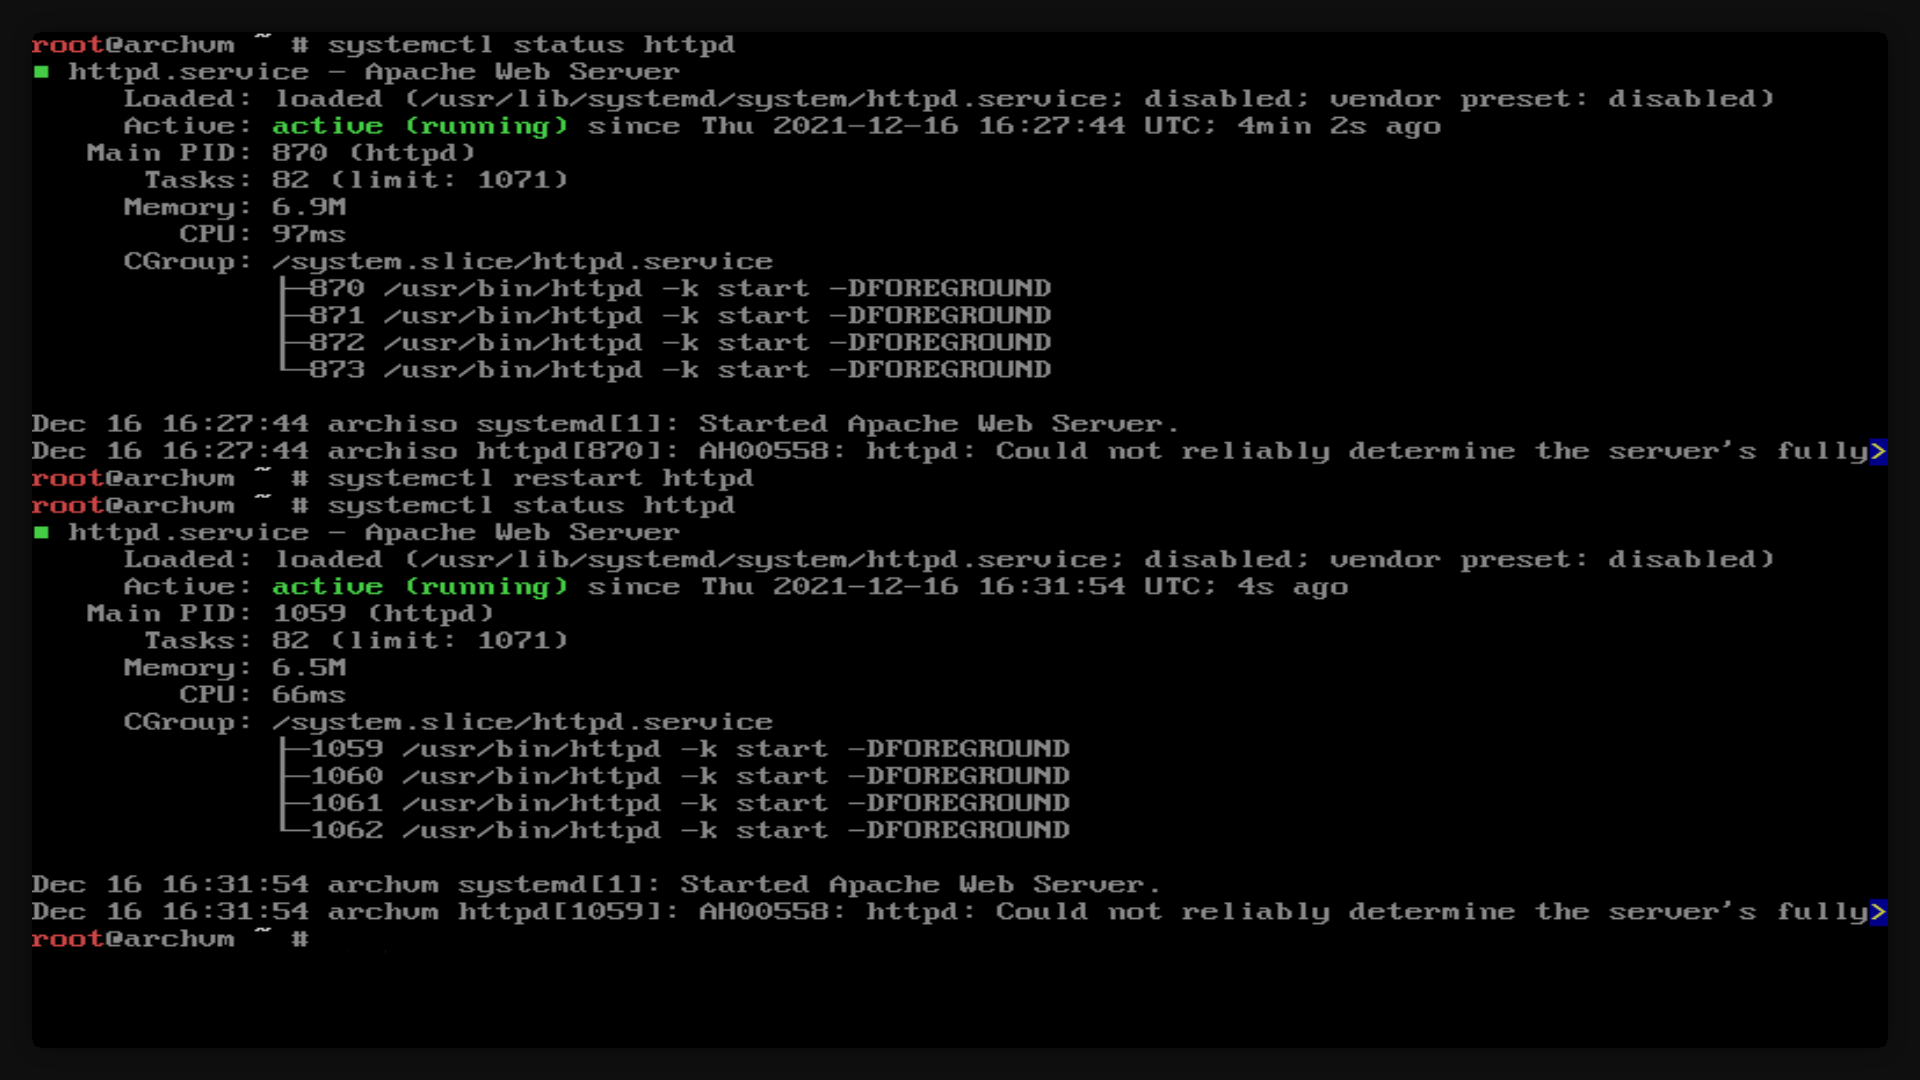
\includegraphics[width=\textwidth,clip=true]{img/1.png}
			\caption{Проверяем работу службы httpd и перезапускаем ее}
		\end{figure}

		\begin{figure}[H]
			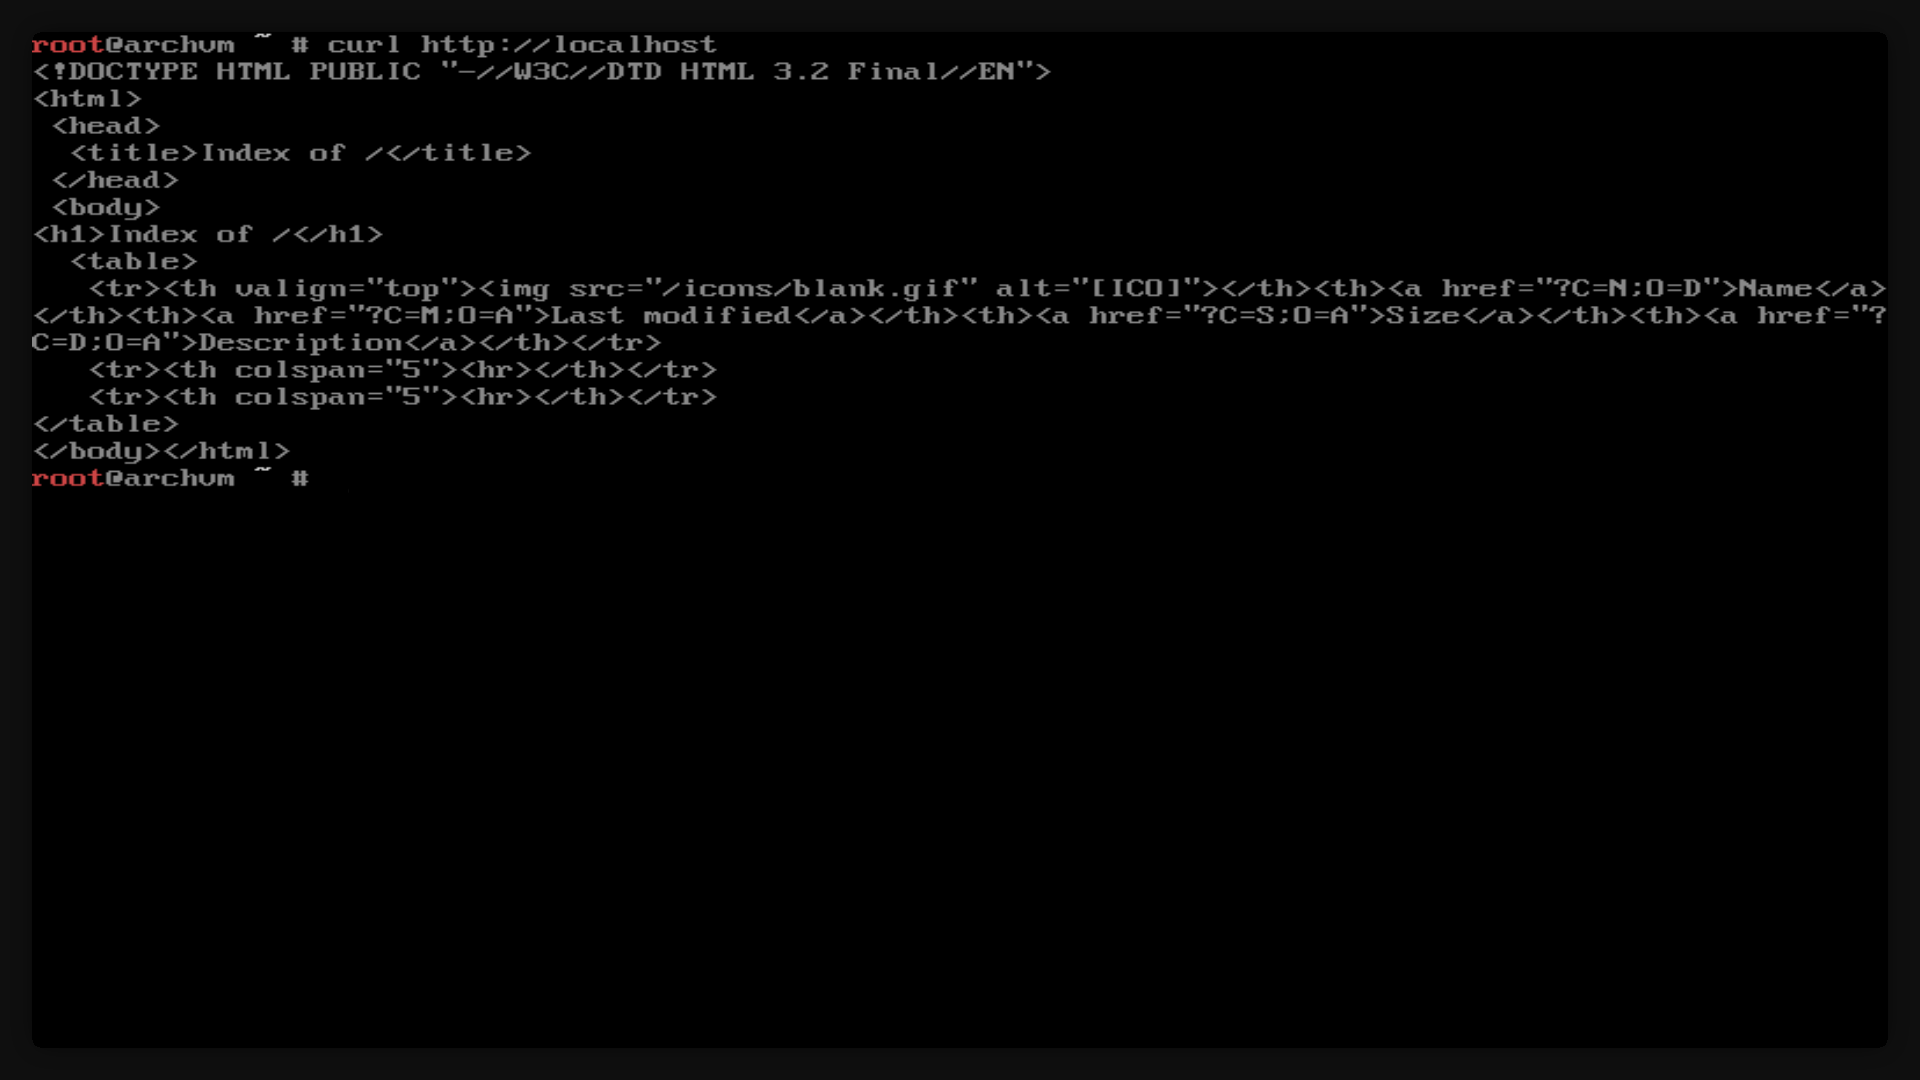
\includegraphics[width=\textwidth,clip=true]{img/2.png}
			\caption{Проверяем работу сервера Apache с помощью curl в гостевой системе}
		\end{figure}

		\begin{figure}[H]
			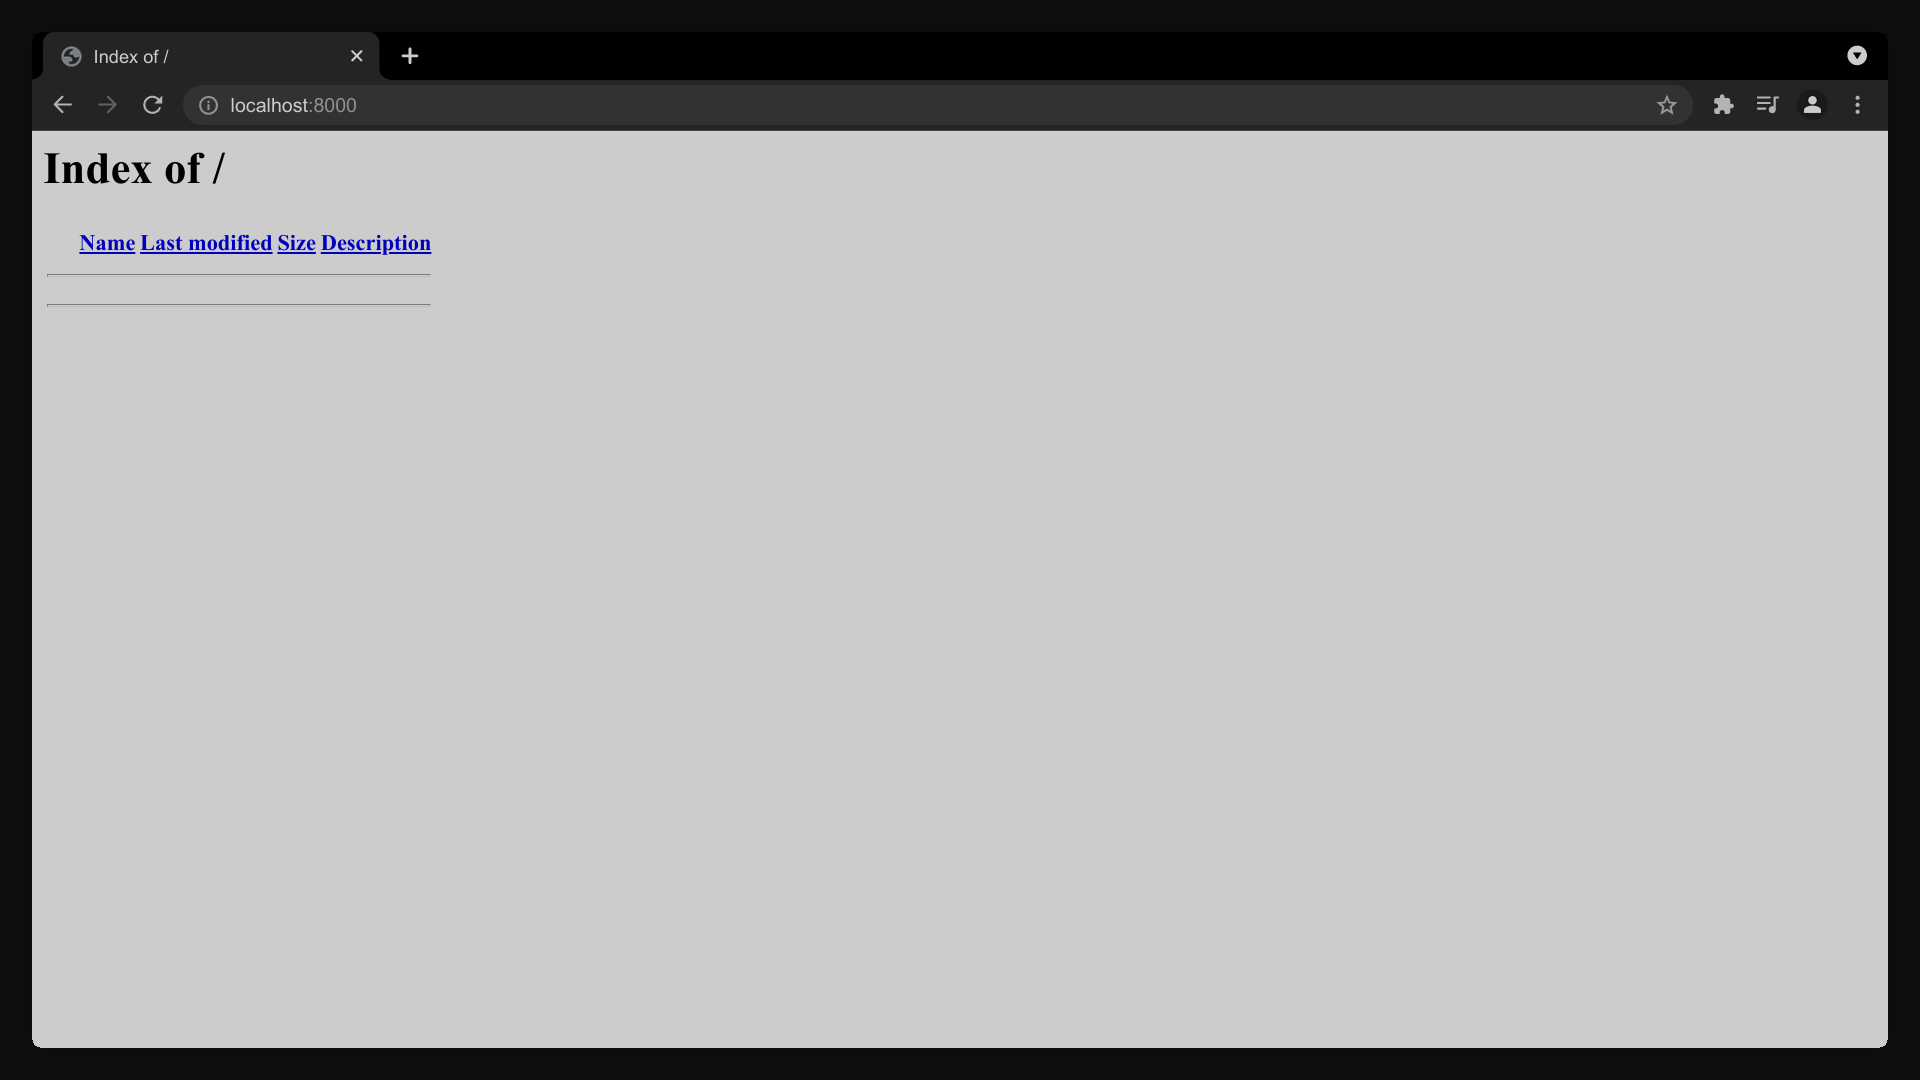
\includegraphics[width=\textwidth,clip=true]{img/3.png}
			\caption{Проверяем работу сервера Apache в браузере в основной системе
			(порт 80 в гостевой ОС проброшен на порт 8000)}
		\end{figure}

	\section{Создание пользователей и групп}
		\begin{figure}[H]
			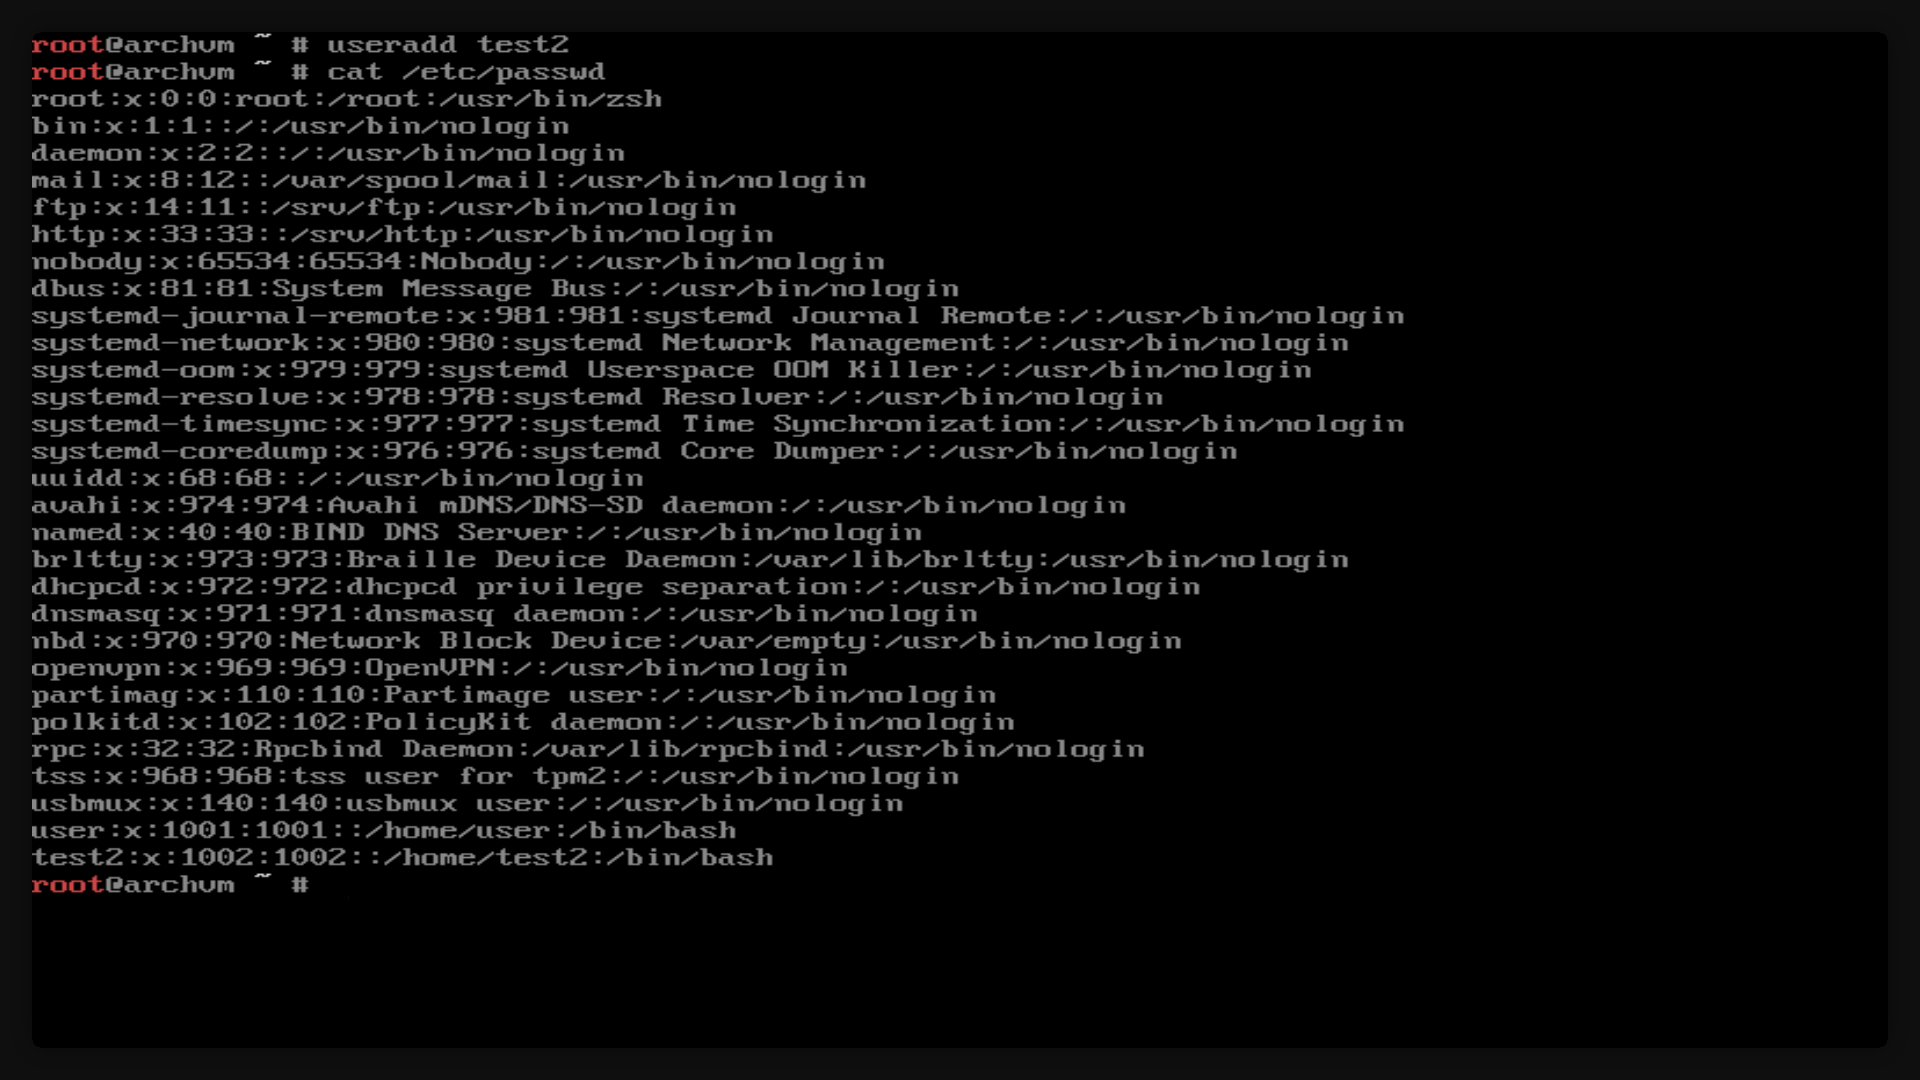
\includegraphics[width=\textwidth,clip=true]{img/4.png}
			\caption{Создаем пользователя test1 и проверяем его наличие в файле
			/etc/passwd}
		\end{figure}

		\begin{figure}[H]
			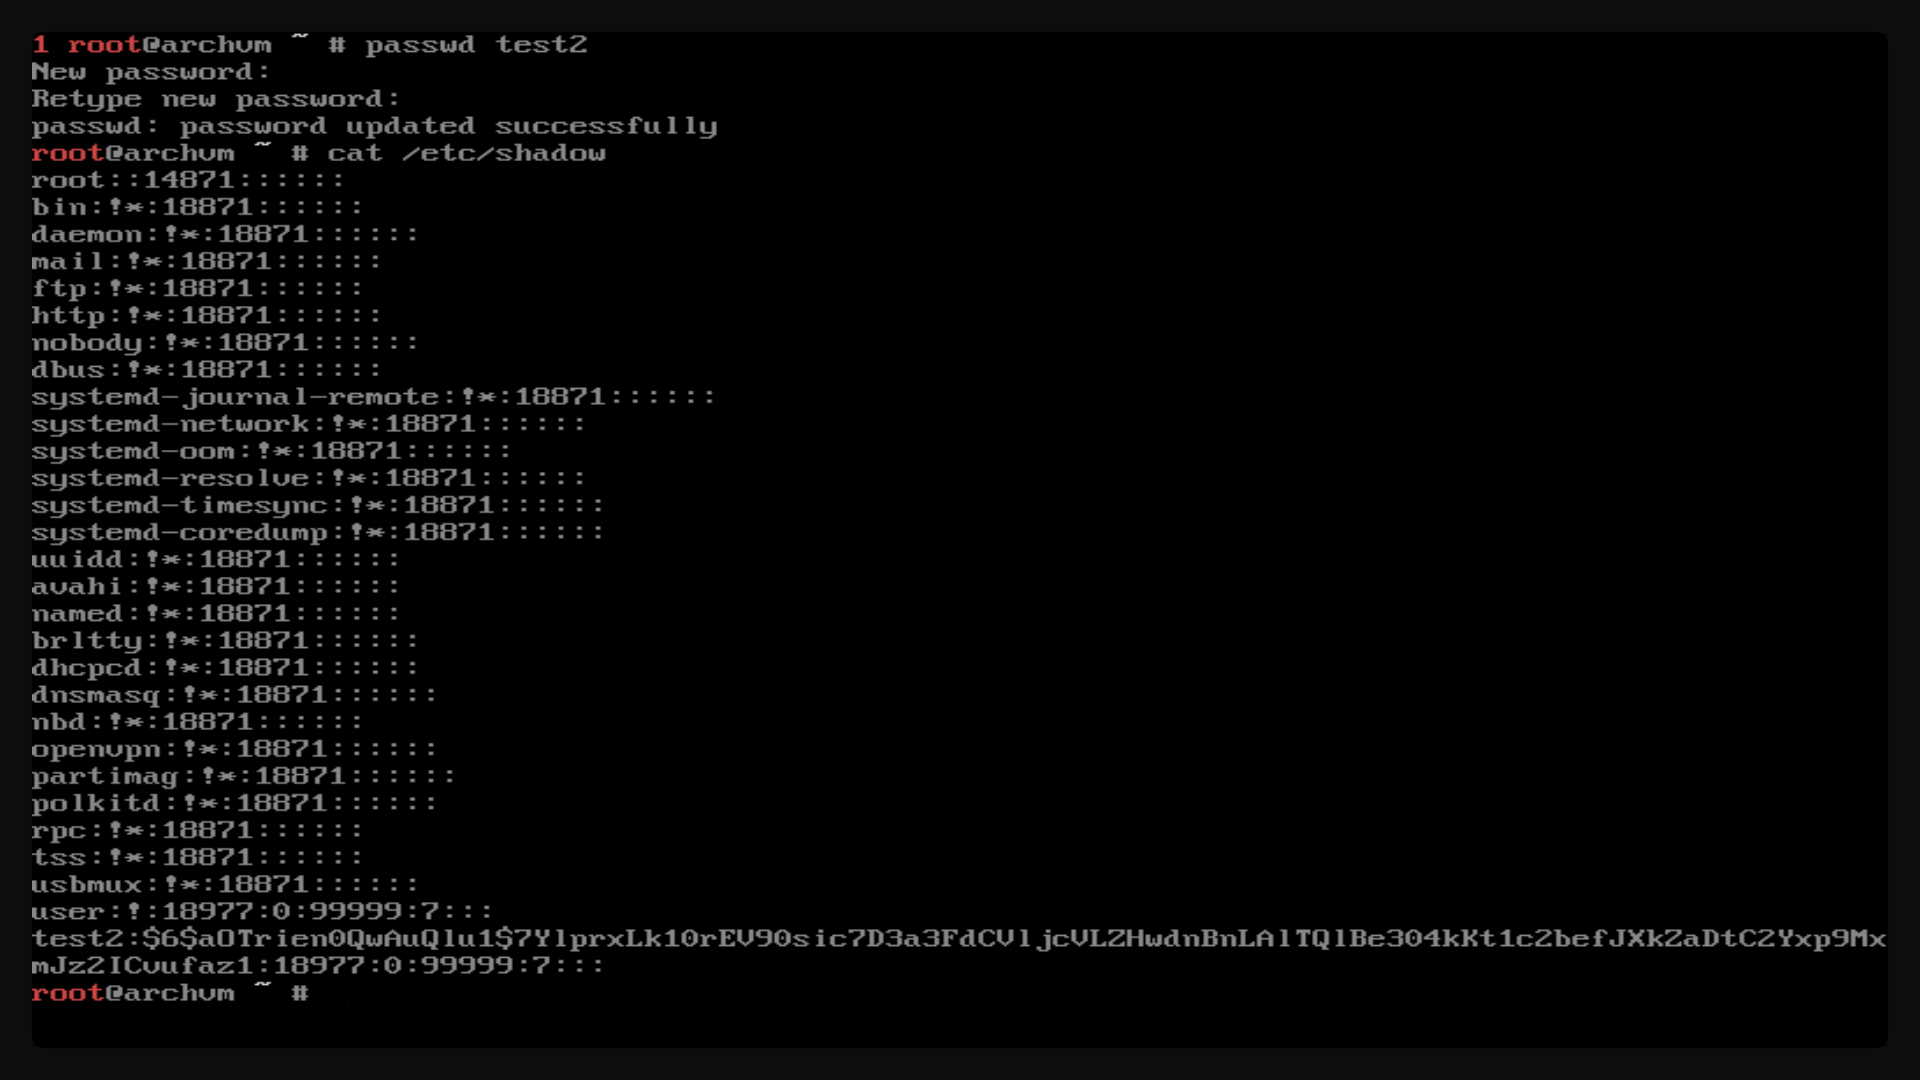
\includegraphics[width=\textwidth,clip=true]{img/5.png}
			\caption{Задаем пользователю test2 пароль и проверяем его в файле
			/etc/shadow}
		\end{figure}

		\begin{figure}[H]
			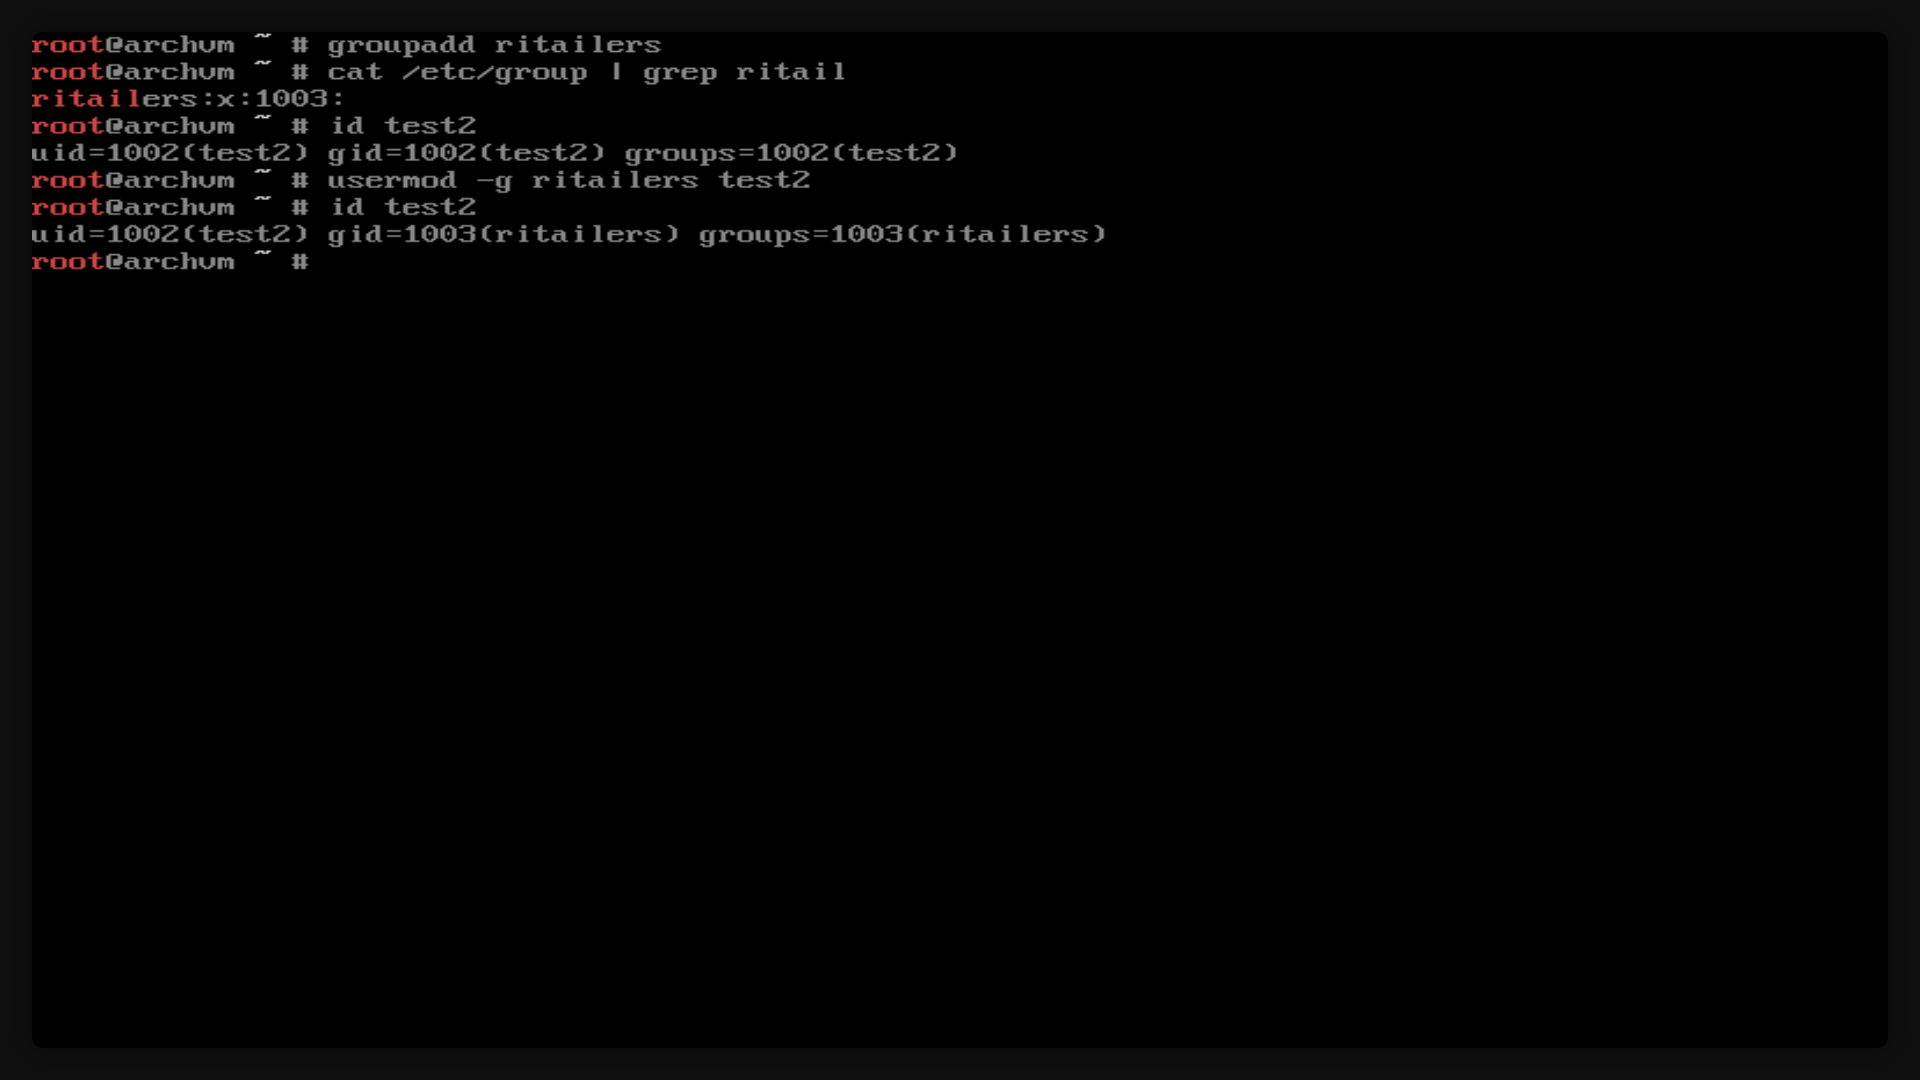
\includegraphics[width=\textwidth,clip=true]{img/6.png}
			\caption{Создаем группу ritailers и добавляем в нее пользователя test2}
		\end{figure}
\end{document}
